% =========================================================
% SUBIR ESTE CÓDIGO COMO CAPÍTULO DE PRÁCTICA EN LA MEMORIA
% =========================================================
\chapter{Cuaderno de Laboratorio — Práctica 3: Metodología de Evaluación y Rigor Científico}

\section*{Objetivo}
Aprender a realizar evaluaciones honestas en condiciones difíciles, especialmente con datos desbalanceados,
y detectar errores metodológicos graves como la fuga de datos (\textit{data leakage}).

\section*{Material de partida}
Se parte de:
\begin{itemize}
    \item Un dataset sintético de \textbf{1000 pacientes} con \textbf{5 variables predictoras}.
    \item Una clase positiva muy minoritaria (\textbf{2\%} de los casos).
\end{itemize}

\section{Tarea 1 — La lotería de la partición aleatoria}

\subsection*{Configuración común}
Modelo usado: \underline{\hspace{6cm}}\\
Métricas usadas: \underline{\hspace{5cm}}\\
Semilla(s): \underline{\hspace{8cm}}

\vspace{0.3cm}
\noindent\textbf{Hipótesis inicial (antes de ejecutar):}
¿Crees que el número de positivos en test será estable? ¿Por qué?
\vspace{1.2cm}

\subsection{Registro de resultados (5 particiones aleatorias)}
\begin{center}
\begin{tabular}{|c|c|}
\hline
Ejecución & Positivos en test \\
\hline
1 & \underline{\hspace{2.5cm}} \\
2 & \underline{\hspace{2.5cm}} \\
3 & \underline{\hspace{2.5cm}} \\
4 & \underline{\hspace{2.5cm}} \\
5 & \underline{\hspace{2.5cm}} \\
\hline
\end{tabular}
\end{center}

\begin{center}
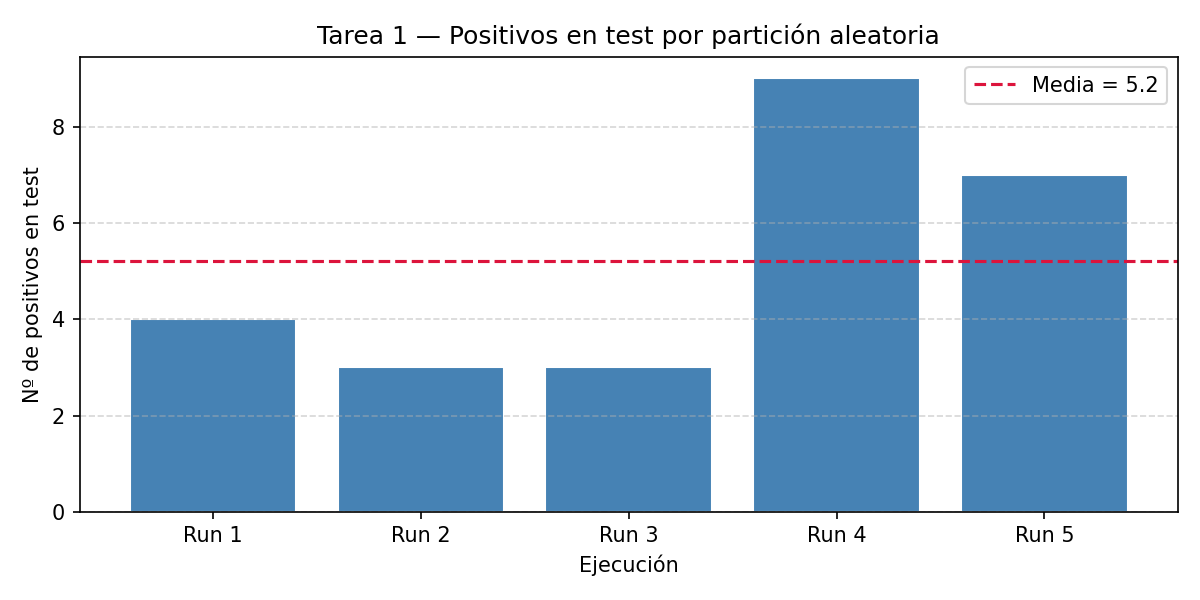
\includegraphics[width=0.85\linewidth]{outputs/tarea1_positivos_test_aleatorio.png}
\end{center}

\noindent\textbf{Análisis:}
\begin{itemize}
    \item ¿Ha cambiado mucho el número de positivos en test entre ejecuciones?
    \item ¿Sería fiable la evaluación si el azar dejara solo 0 o 1 positivos en test?
\end{itemize}

\vspace{1.5cm}

\section{Tarea 2 — Partición estratificada}

\subsection{Registro por folds}
\begin{center}
\begin{tabular}{|c|c|c|c|}
\hline
Fold & Positivos en test & Tamaño del fold & Proporción clase 1 \\
\hline
1 & \underline{\hspace{1.8cm}} & \underline{\hspace{1.8cm}} & \underline{\hspace{2.0cm}} \\
2 & \underline{\hspace{1.8cm}} & \underline{\hspace{1.8cm}} & \underline{\hspace{2.0cm}} \\
3 & \underline{\hspace{1.8cm}} & \underline{\hspace{1.8cm}} & \underline{\hspace{2.0cm}} \\
4 & \underline{\hspace{1.8cm}} & \underline{\hspace{1.8cm}} & \underline{\hspace{2.0cm}} \\
5 & \underline{\hspace{1.8cm}} & \underline{\hspace{1.8cm}} & \underline{\hspace{2.0cm}} \\
\hline
\end{tabular}
\end{center}

\begin{center}
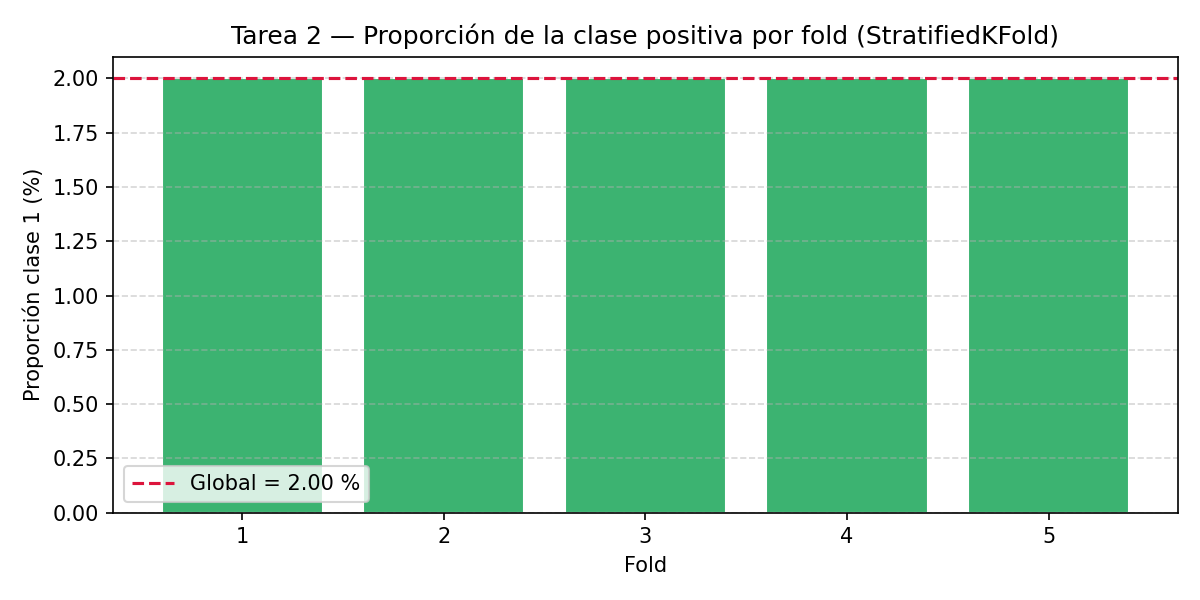
\includegraphics[width=0.85\linewidth]{outputs/tarea2_proporcion_folds_estratificado.png}
\end{center}

\noindent\textbf{Análisis:}
Explica por qué \texttt{StratifiedKFold} es más adecuado que una partición aleatoria simple en este problema.
\vspace{1.6cm}

\section{Tarea 3 — Comparativa de la varianza}

\subsection{Resumen de resultados}
\begin{center}
\begin{tabular}{|c|c|c|c|c|}
\hline
Método & Accuracy media & std(Accuracy) & F1 media & std(F1) \\
\hline
KFold & \underline{\hspace{2cm}} & \underline{\hspace{2cm}} & \underline{\hspace{2cm}} & \underline{\hspace{2cm}} \\
StratifiedKFold & \underline{\hspace{2cm}} & \underline{\hspace{2cm}} & \underline{\hspace{2cm}} & \underline{\hspace{2cm}} \\
\hline
\end{tabular}
\end{center}

\begin{center}
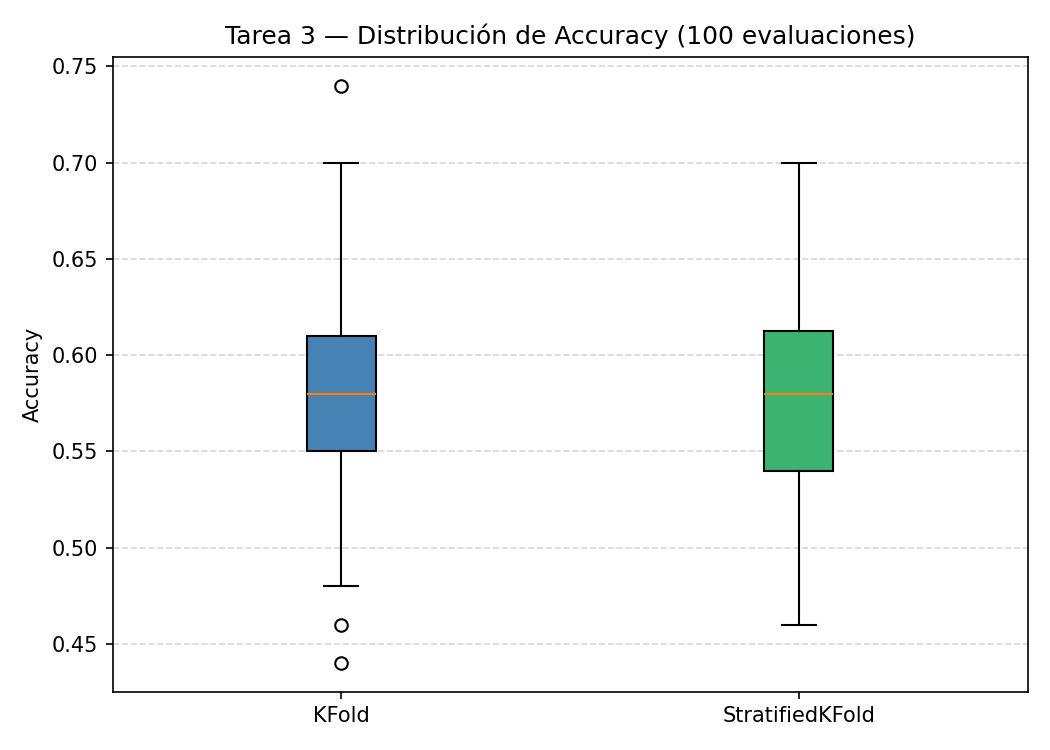
\includegraphics[width=0.85\linewidth]{outputs/tarea3_boxplot_accuracy.png}
\end{center}

\begin{center}
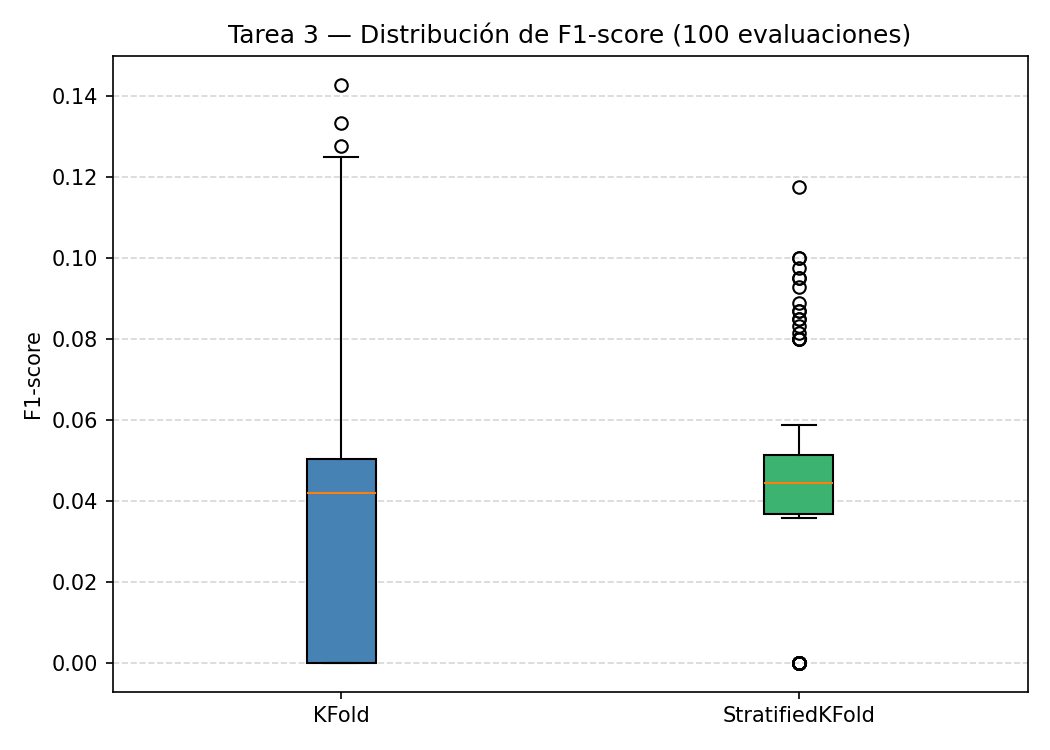
\includegraphics[width=0.85\linewidth]{outputs/tarea3_boxplot_f1.png}
\end{center}

\noindent\textbf{Interpretación:}
\begin{itemize}
    \item ¿Qué método produce métricas más estables?
    \item ¿Dónde se nota más la mejora, en Accuracy o en F1?
\end{itemize}

\vspace{1.4cm}

\section{Tarea 4 — Detección de data leakage}

\subsection{Comparativa}
\begin{center}
\begin{tabular}{|c|c|c|}
\hline
Escenario & Accuracy & F1 \\
\hline
Sin variable trampa & \underline{\hspace{2cm}} & \underline{\hspace{2cm}} \\
Con variable trampa & \underline{\hspace{2cm}} & \underline{\hspace{2cm}} \\
\hline
\end{tabular}
\end{center}

\begin{center}
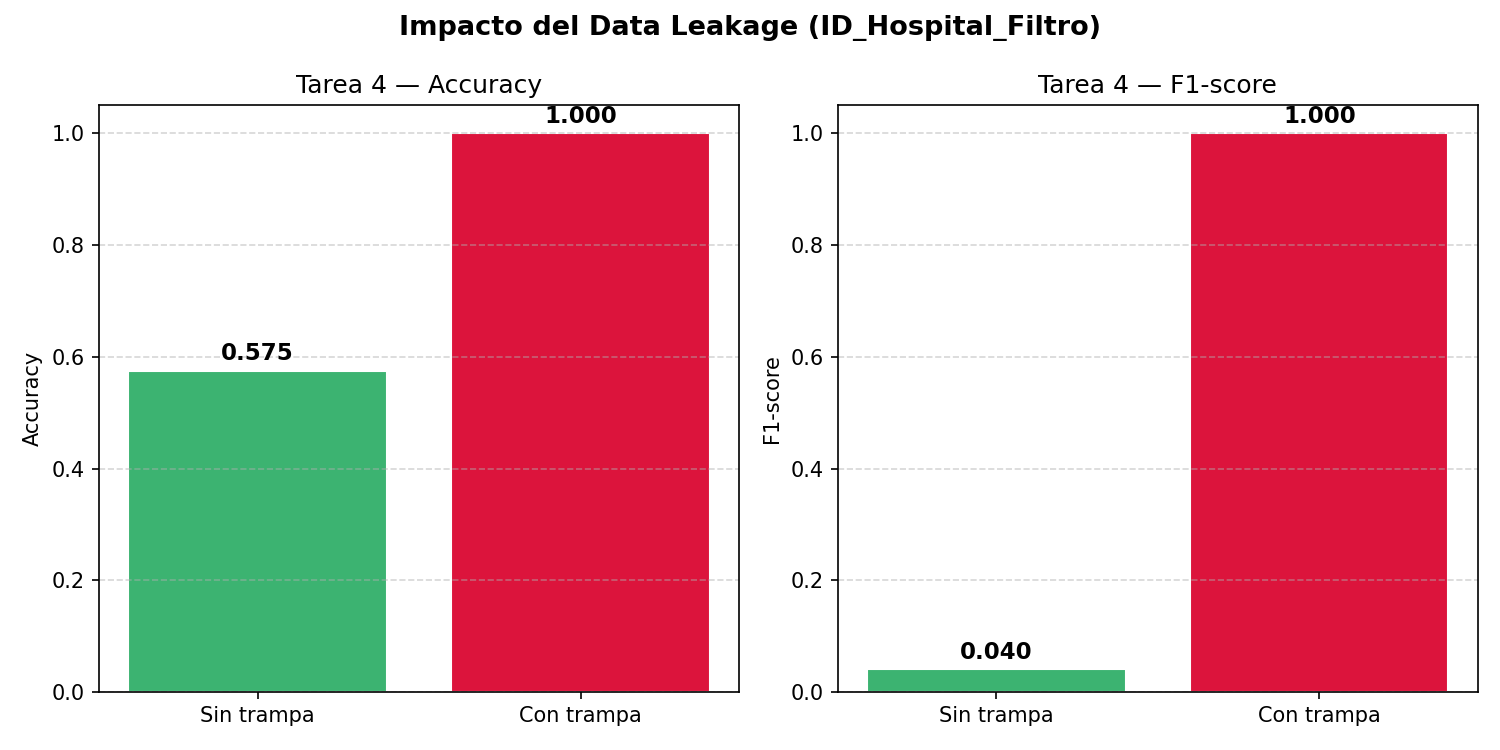
\includegraphics[width=0.85\linewidth]{outputs/tarea4_accuracy_leakage.png}
\end{center}

\begin{center}
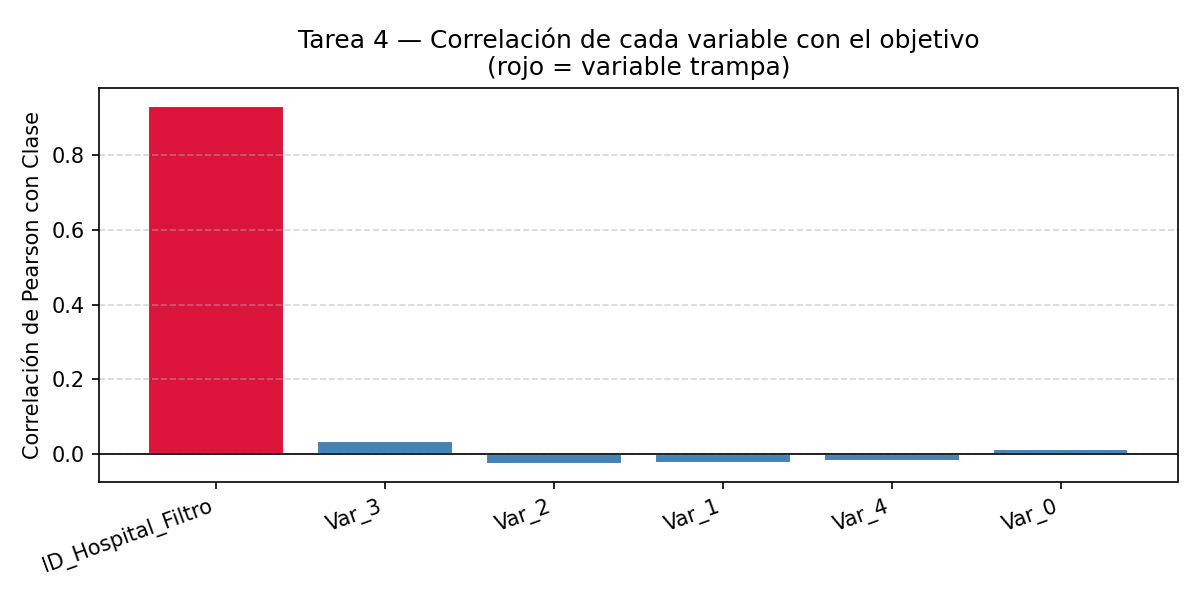
\includegraphics[width=0.90\linewidth]{outputs/tarea4_correlaciones_leakage.png}
\end{center}

\noindent\textbf{Preguntas:}
\begin{itemize}
    \item ¿Qué variable sospechas que está filtrando información del objetivo?
    \item ¿Por qué esa variable invalida la evaluación?
    \item ¿Qué diferencia conceptual hay entre un modelo ``bueno'' y un modelo contaminado por leakage?
\end{itemize}

\vspace{1.4cm}

\section{Reto — Auditoría metodológica}
Redacta un pequeño informe (6--10 líneas) respondiendo a estas cuestiones:
\begin{enumerate}
    \item ¿Por qué una partición aleatoria simple puede ser peligrosa en problemas desbalanceados?
    \item ¿Qué aporta la validación estratificada?
    \item ¿Por qué el \textit{data leakage} puede hacer inútiles las conclusiones de un experimento?
    \item ¿Qué buenas prácticas metodológicas seguirías en futuros experimentos?
\end{enumerate}

\vspace{2cm}

\section{Conclusión final}
Resume qué has aprendido sobre evaluación rigurosa, estabilidad de métricas y detección de errores metodológicos.
